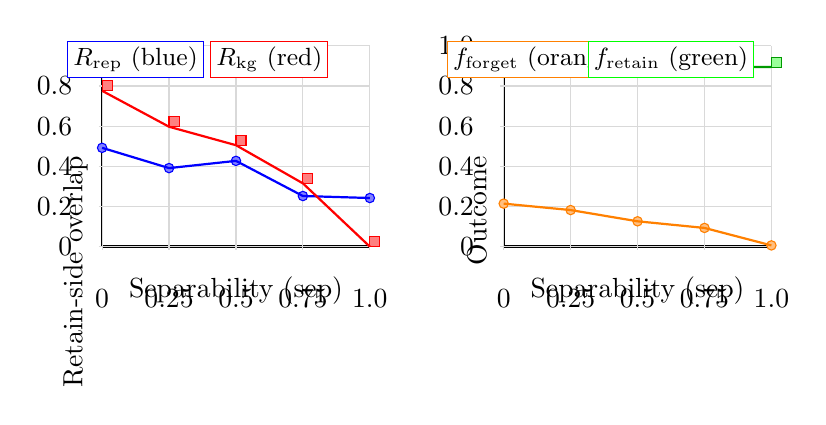
\begin{tikzpicture}[scale=0.85]
  % Left plot: retain-side overlap
  \draw[thick] (0,0) -- (4,0);
  \draw[thick] (0,0) -- (0,3);

  \node[below] at (2,-0.3) {Separability ($\mathrm{sep}$)};
  \node[left,rotate=90] at (-0.4,1.5) {Retain-side overlap};

  % Grid lines
  \foreach \x in {0,1,2,3,4} \draw[gray!30] (\x,-0.05) -- (\x,3);
  \foreach \y in {0,0.6,1.2,1.8,2.4,3} \draw[gray!30] (-0.05,\y) -- (4,\y);

  % X-axis labels
  \node[below] at (0,-0.5) {0};
  \node[below] at (1,-0.5) {0.25};
  \node[below] at (2,-0.5) {0.5};
  \node[below] at (3,-0.5) {0.75};
  \node[below] at (4,-0.5) {1.0};

  % Y-axis labels
  \node[left] at (-0.3,0) {0};
  \node[left] at (-0.3,0.6) {0.2};
  \node[left] at (-0.3,1.2) {0.4};
  \node[left] at (-0.3,1.8) {0.6};
  \node[left] at (-0.3,2.4) {0.8};

  % R_rep data (blue circles): 0.492, 0.391, 0.427, 0.252, 0.242
  \foreach \x/\y in {0/1.476, 1/1.173, 2/1.281, 3/0.756, 4/0.726} {
    \filldraw[blue!50, draw=blue] (\x,\y) circle (2pt);
  }
  \draw[blue, thick] (0,1.476) -- (1,1.173) -- (2,1.281) -- (3,0.756) -- (4,0.726);

  % R_kg data (red squares): 0.776, 0.597, 0.505, 0.315, 0.000
  \foreach \x/\y in {0/2.328, 1/1.791, 2/1.515, 3/0.945, 4/0} {
    \filldraw[red!50, draw=red] (\x,\y) rectangle (\x+0.15,\y+0.15);
  }
  \draw[red, thick] (0,2.328) -- (1,1.791) -- (2,1.515) -- (3,0.945) -- (4,0);

  % Legend
  \node[draw=blue, fill=white, inner sep=2pt] at (0.5,2.8) {\small $R_{\mathrm{rep}}$ (blue)};
  \node[draw=red, fill=white, inner sep=2pt] at (2.5,2.8) {\small $R_{\mathrm{kg}}$ (red)};

  % =====================================================

  % Right plot: Outcome (shifted)
  \begin{scope}[xshift=6cm]
    \draw[thick] (0,0) -- (4,0);
    \draw[thick] (0,0) -- (0,3);

    \node[below] at (2,-0.3) {Separability ($\mathrm{sep}$)};
    \node[left,rotate=90] at (-0.4,1.5) {Outcome};

    % Grid lines
    \foreach \x in {0,1,2,3,4} \draw[gray!30] (\x,-0.05) -- (\x,3);
    \foreach \y in {0,0.6,1.2,1.8,2.4,3} \draw[gray!30] (-0.05,\y) -- (4,\y);

    % X-axis labels
    \node[below] at (0,-0.5) {0};
    \node[below] at (1,-0.5) {0.25};
    \node[below] at (2,-0.5) {0.5};
    \node[below] at (3,-0.5) {0.75};
    \node[below] at (4,-0.5) {1.0};

    % Y-axis labels
    \node[left] at (-0.3,0) {0};
    \node[left] at (-0.3,0.6) {0.2};
    \node[left] at (-0.3,1.2) {0.4};
    \node[left] at (-0.3,1.8) {0.6};
    \node[left] at (-0.3,2.4) {0.8};
    \node[left] at (-0.3,3) {1.0};

    % f_forget data (orange circles): 0.214, 0.182, 0.126, 0.093, 0.006
    \foreach \x/\y in {0/0.642, 1/0.546, 2/0.378, 3/0.279, 4/0.018} {
      \filldraw[orange!50, draw=orange] (\x,\y) circle (2pt);
    }
    \draw[orange, thick] (0,0.642) -- (1,0.546) -- (2,0.378) -- (3,0.279) -- (4,0.018);

    % f_retain data (green squares): 0.953, 0.965, 0.941, 0.898, 0.894
    \foreach \x/\y in {0/2.859, 1/2.895, 2/2.823, 3/2.694, 4/2.682} {
      \filldraw[green!40, draw=green!60!black] (\x,\y) rectangle (\x+0.15,\y+0.15);
    }
    \draw[green!60!black, thick] (0,2.859) -- (1,2.895) -- (2,2.823) -- (3,2.694) -- (4,2.682);

    % Legend
    \node[draw=orange, fill=white, inner sep=2pt] at (0.5,2.8) {\small $f_{\mathrm{forget}}$ (orange)};
    \node[draw=green, fill=white, inner sep=2pt] at (2.5,2.8) {\small $f_{\mathrm{retain}}$ (green)};
  \end{scope}
\end{tikzpicture}
